\chapter{Introduction}
\label{chap:introduction}

Taking inspiration from the fascinating natural phenomena of self synchronizing fireflies, as e.g. seen in Figure \ref{fig:synched_fireflies_phenomenon}, a synchronization simulator imitating and modelling this process for—instead of fireflies—a collective of musical robots, as e.g. seen in Figure \ref{fig:illustrative_developed_system}, has been designed and tested.

The effects, particularly in terms of the ability to and performance of synchronization, is measured and evaluated when experimentally altering the properties of the musical robot collective as a whole (as e.g. collective size), or individual musical robots's hyperparameters (e.g. the number of neighbouring robots each robot listens to for self synchronization).

\begin{figure}[!ht]
	\centering
	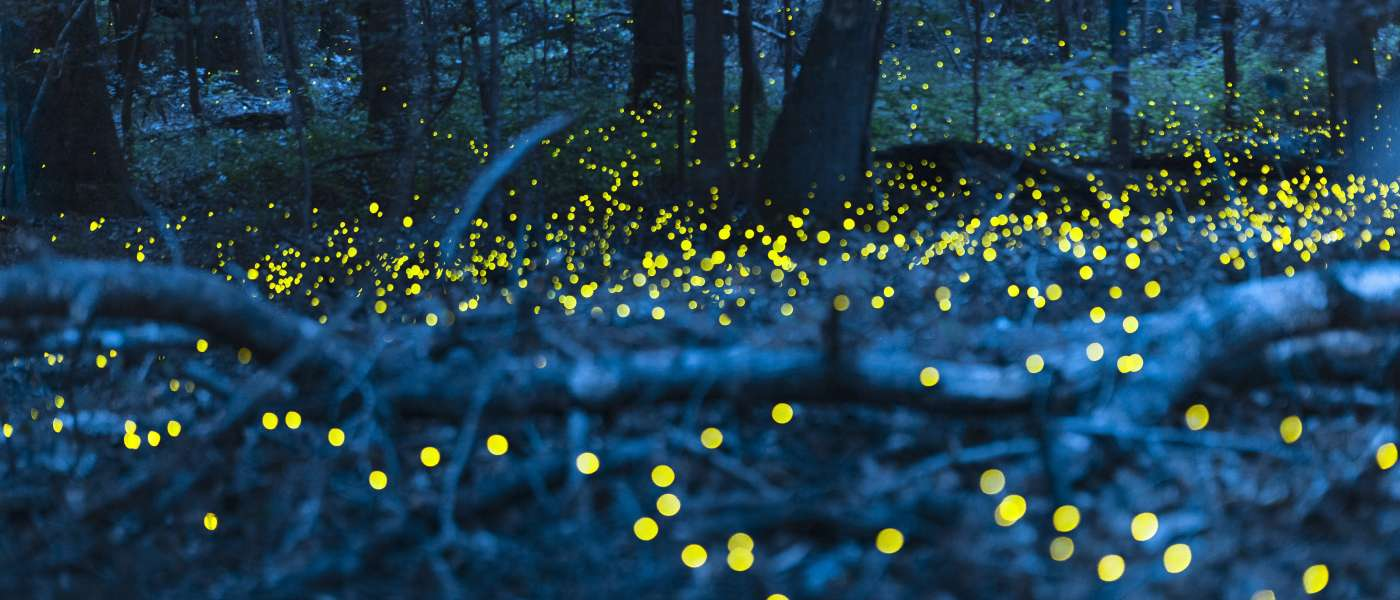
\includegraphics[width=\linewidth]{Assets/DocSegments/Chapters/Background/Figures/Photos/synchronized_fireflies_phenomenon.jpg}
	\caption[Picture of fireflies flashing synchronously in a US National Park]{Synchronous fireflies at Congaree National Park, United States. Photo\protect\footnotemark: @columbiasc \& @\_flashnick.} % ELLER F.EKS. {Copyright ©Blabla Corporation, David Thorvaldsen}
	\label{fig:synched_fireflies_phenomenon}
\end{figure}

\footnotetext{\url{https://avltoday.6amcity.com/synchronous-fireflies-congaree-national-park/} (accessed 2022.05.17)}

\np

\begin{figure}[!ht]
  \begin{subfigure}[b]{0.495\textwidth}
	\centering\captionsetup{width=.9\linewidth}%
	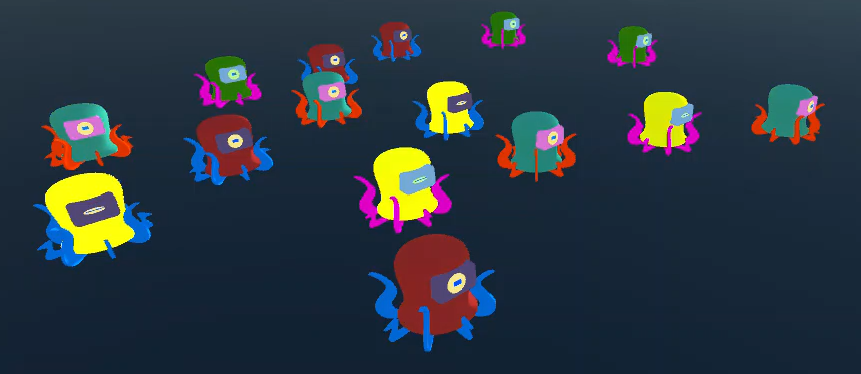
\includegraphics[width=\textwidth]{Assets/DocSegments/Chapters/Introduction/Figures/illustrative_system_result_figure_s0p8.png}
	\caption{0.8 seconds after simulation start.}
	\label{fig:sub:illustrative_developed_system_t1}
  \end{subfigure}
  %
  \begin{subfigure}[b]{0.495\textwidth}
	\centering\captionsetup{width=.9\linewidth}%
	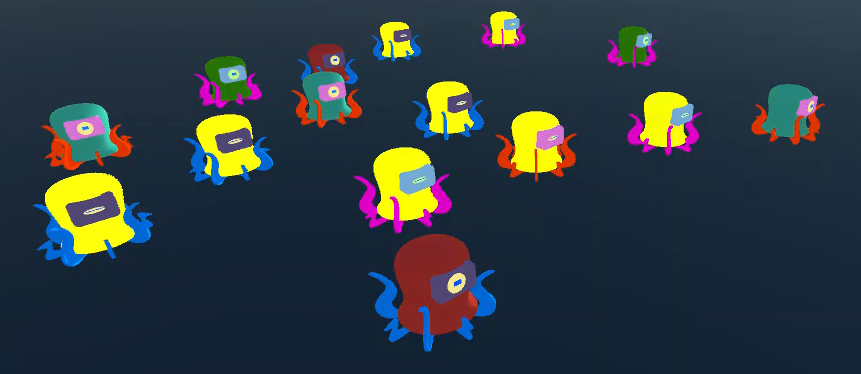
\includegraphics[width=\textwidth]{Assets/DocSegments/Chapters/Introduction/Figures/illustrative_system_result_figure_s2p3.png}
	\caption{2.3 seconds after simulation start.}
	\label{fig:sub:illustrative_developed_system_t2}
  \end{subfigure}
  \begin{subfigure}[b]{0.495\textwidth}
	\centering\captionsetup{width=.9\linewidth}%
	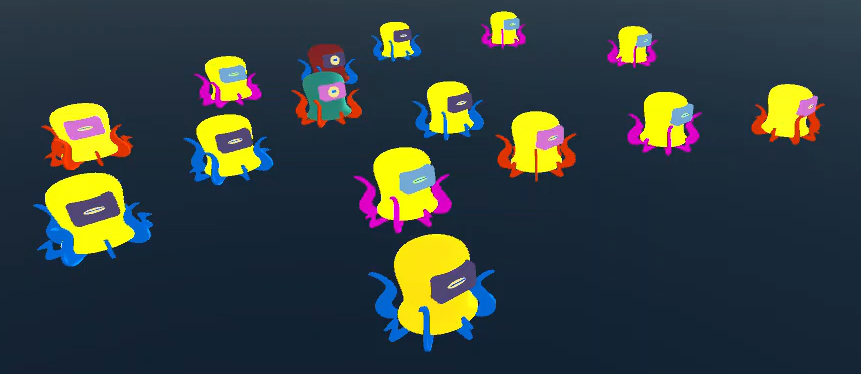
\includegraphics[width=\textwidth]{Assets/DocSegments/Chapters/Introduction/Figures/illustrative_system_result_figure_s6p2.png}
	\caption{6.2 seconds after simulation start.}
	\label{fig:sub:illustrative_developed_system_t3}
  \end{subfigure}
  %
  \begin{subfigure}[b]{0.495\textwidth}
	\centering\captionsetup{width=.9\linewidth}%
	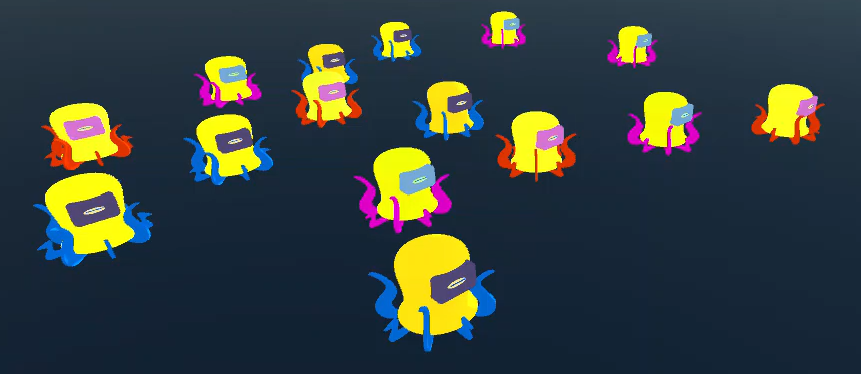
\includegraphics[width=\textwidth]{Assets/DocSegments/Chapters/Introduction/Figures/illustrative_system_result_figure_s10p1.png}
	\caption{10.1 seconds after simulation start.}
	\label{fig:sub:illustrative_developed_system_t4}
  \end{subfigure}
  \caption[Developed synchronization simulator inspired by synchronously flashing fireflies.]{A typical simulation run of a musical multi robot collective (here of size 15) entraining to achieve harmonic synchronization in the developed system. As we can see\protect\footnotemark, the robots start flashing yellow and blinking with their eyes asynchronously at first in \ref{fig:sub:illustrative_developed_system_t1}, but end up synchronized in \ref{fig:sub:illustrative_developed_system_t4}. Due to our special synchronization type being \textit{harmonic synchronization} (cf. \ref{sec:harmonic_synchrony}), as well as an implementation choice of robots only ``flashing'' or ``firing'' every other phase climax (i.e. $\phi=1$), musical robot collectives do not in fact have to all fire simultaneously in order to be harmonically synchronized, but all robots firing simultaneously is also a validly harmonically synchronized robot collective.}
  \label{fig:illustrative_developed_system}
\end{figure}

\footnotetext{See video at \url{https://www.uio.no/ritmo/english/projects/modeling-and-robots/media/phasesyncrecord.mp4} (accessed 2022.05.27)}




\section{Motivation}

% Introducing challenges concerning knowledge and communication in (autonomous) computing systems given extreme and challenging environments:

Engineering a computing system for a certain environment often requires some knowledge of said environment; both on the end of the system-creator, as well as for the computing system in turn. This knowledge will then have to be used in the environment the computing system is situated in, in all the situations and possible states the system can be in during its lifetime. However, foreseeing and predicting, at design-time, all possible future states and scenarios a computing system will be in during its lifetime is often hard, and sometimes impossible (in the case of coincidental faults e.g.). Increasingly extreme, complex, dynamic, and ever-changing environments, simply enlargens this challenge.

Extreme challenges and physical barriers within communication between decentralized and mobile robots and its human operator, like too large latencies, bottlenecks presented by using the same limited bandwidths, short possible ranges, or the inability to use global satellite systems e.g. in underwater vehicles \cite{petillot_underwater_robots}, leads to the necessity of enabling systems to autonomously and online control themselves and perform missions without communication from remote operators like humans. This calls for online and continuous learning at run time, where computing systems are themselves able to observe, learn, adapt, and act on their own, independently from their creator; \textit{autonomic computing} that is. Hence, technological development and research has e.g. within underwater robotics gone from enabling remotely operated vehicles (ROVs) in the 1980s (for e.g. oil and gas exploitation at depths unreachable to human divers), over to more self adaptive and autonomous underwater vehicles (AUVs) closer to in the 21st century —the demand of which is expected to grow 37\% in the 2018-2022 period \cite{petillot_underwater_robots}. As a result, the underwater robots can in this instance thus, due to the increased degree of autonomy and consequently implicit reduction in communication need, travel on its own on even longer and extensive missions without the need for a live connection to any human operator—e.g. on seabed mapping missions, underwater machinery or structure maintenance, as well as seabed cleaning.

% Transitioning from autonomous agents to synchronizing oscillators:

However, and especially within collectives of multiple robots \cite{cocoro, swarm_bot}, communication between individuals—even though they might be autonomous individual robots—is still a challenge one has to deal with when designing them. Coordination, for humans and robots alike, often tend to demand a lot of communication. To add on top of this, when networks or collectives of sub-systems like wireless sensors are communicating with each other, they often have their own internal clock which often do not align. Hence, we see that both the magnitude of communication needed, as well as the inherent challenges with communication, call for effective approaches to communication with coordination as the goal.

As K. Konishi \& H. Kokame \cite{konishi_kokame} points out, one technical problem in e.g. wireless sensor networks is that each sensor node rely on accurate internal and synchronized clocks, especially from the perspective of sensor fusion and coordinating communication among nodes. Thus, time synchronization becomes recognized as one of the crucial problems in distributed and wireless systems \cite{tungvinte_sync_protocols}. Various attempts at synchronizing messages and communication, in order to e.g. align messages exchanged at unsynchronized intervals, have been made \cite{tungvinte_sync_protocols}; however, such attempts and protocols often require the computation of message exchange and processing, which wastes the limited computation capability of nodes and causes communication delays. To this, Konishi \& Kokame \cite{konishi_kokame} also point out how for synchronized pulse coupled oscillators (PCOs), such computation is not required. If internal clocks in communicating nodes are instead altered and synchronized to other nodes's clocks—instead of letting all clocks stay unsynchronized and constantly trying to compensate for this— it is rather apparent that getting rid of this need for compensation will considerably reduce computation needs while synchronized communication is still achieved.

Thus, by achieving time synchronization \cite{tungvinte_sync_protocols} through synchronizing pulse coupled oscillators, both the computational load, in addition to the need for communication, is considerably reduced; hence freeing up and saving valuable resources like e.g. processing power and energy (battery) in networks of individuals and possibly autonomous nodes, agents, or robots.


% SA + decentralized and autonomous (musical) robots / agents + Oscillator sync = <3 :

On another hand, self-awareness concepts from psychology have given inspiring new approaches for engineering computing systems which operate in complex dynamic environments \cite{sacs16_ch2}. As we can see in various Music Technology Systems, this endowing can also give rise to interesting cooperative and coordinating behaviour.

With self awareness, online and continuous learning is achieved to a higher degree in contrast with other approaches (like ODA and MAPE-K), due to the limitations and downsides of these older approaches, as well as the advantages and upsides to considering computational self-awareness in computing systems. If one wants to achieve continuous adaptation of a system or of system-components (e.g. in a collective) — some sort of intelligence might be necessary to endow it with. Endowing computing systems with Self-Awareness can be beneficial in several respects, including but not limited to a greater capacity to adapt, to build potential for future adaptation in unknown environments, and to explain their behaviour to humans and other systems \cite{sacs17_ch3}.

Explainability has with time only become more and more relevant, also within artificial intelligence (AI) (hence the popularity of the term \textit{explainable AI}), as increasingly autonomous and automatically systems are making real life decisions with serious consequences increasingly on a day to day basis. L. A. Dennis and M. Fisher present explaining and verifiable agent-based systems, where rational agents who possess goals, beliefs, desires, intentions e.g. make decisions that in their opinion should be able to be questioned and giving an answer when prompted \cite{verifiable_and_questionable_agents}. Self awareness enables such questioning and answering by autonomous agents, as the agents themselves, since they are themselves aware of their knowledge, thoughts, goals, desires etc., can explain what lead to their actions. Or in other words, questions like ``what type of self awareness \cite{sacs16_ch2} (knowledge) lead to a certain self expression \cite{sacs16_ch2} (action)'' can be answered by self aware and self expressive agents. Such an example can be read by P. Lewis et al. \cite{sacs17_ch3} (3.3.4) when they summarize their novel computational self awareness framework by enabling self aware computing systems to produce sentences like the following: Peter (span) is aware of Ada's (scope) goal (aspect) to reduce the power usage (object). Further, Ada (span) is aware of her own reasoning (meta-self-awareness) about what to do (act) about it.

Endowing computing systems with Self-Awareness can be beneficial in several respects, including a greater capacity to adapt, to build potential for future adaptation in unknown environments, and to explain their behaviour to humans and other systems. As we can see in various Music Technology Systems, this endowing can also give rise to interesting cooperative and coordinating behaviour.

% --- \section END. ---



\section{Goal of the thesis} % a.k.a. research goals.

In this MSc-thesis, we will explore an exciting and relatively new translation of the concepts and notions regarding self-awareness — as they pertain to humans and animals especially — from the domain of Psychology, into the domain of computation and engineering. The problem to explore will mainly consist of studying the effects differing self-awareness levels, varying collective-sizes, levels of task difficulty (like more complex behaviours, and limited communication) - have on usefulness, system dynamics, overall performance, more intelligent systems, and scalability (in this case specifically within a musical robot system) when performing a task. Whether the effect of endowing the musical robot system with increased computational self awareness will be better decision making (or \textit{self expression} \cite{sacs16_ch2}), versatility and ability to adapt quickly and online in a rapidly dynamic and everchanging enviroment, as they continually learn by themselves further handling continuous environmental change, or not will be investigated.

Generally, the aim is to discover the effects of endowing computational systems/robots with self-awareness capabilities / abilities. More specifically, the aim of the thesis is to explore and investigate whether—and to which degrees—increased degree or level of computational self awareness in musical robots lead to increased performance in a collective musical task to be achieved; namely, achieving synchronization (\textit{harmonic} at that, cf. \ref{sec:harmonic_synchrony})—much like and inspired by fireflies in nature adjusting and synchronizing themselves and their flashing to each other.

With that, the following research questions is thus introduced, with the hope of answering them in the thesis: \nl

\textbf{Research Question 1}:

To what extent will increased levels or degrees of computational self awareness in individual musical robots lead to the musical collective at large being able to achieve its collective musical task—being (\textit{harmonic}) synchronization—faster compared to with lower levels or degrees of computational self-awareness? \nl

\textbf{Research question 2}:

To what extent can harmonic synchronization performance in musical robot collectives be maintained despite lower degrees or levels of computational self awareness? \nl

\textbf{Research Question 3}:

In what ways do computational systems—specifically a musical robot collective—exhibit and display self awareness (and corresponding self expressive) capabilities, compared to in humans and animals? \nl


% \textbf{Research Question 4}:

% To what degree will increased levels of self-awareness lead to more robustness and flexibility in terms of handling environmental noise and other uncertainties; specifically in the continued ability of musical robots to synchronize to each other efficiently despite these difficult challenges? \nl

% --- \section END. ---



\section{Outline}

The master's thesis is structured as follows. Firstly, past and related work relevant for the thesis will be presented in Chapter \ref{chap:background}, laying the theoretical and inspirational foundation this thesis is basing itself upon.

Then, in Chapter \ref{chap:baseline}, a particularly important and foundational approach to oscillator synchronization is presented in detail, serving as the starting point and baseline for the synchronization method the musical robots in our developed system will utilize in order to achieve the target state also presented and achieved by the authors of the baseline approach.

After the main specific approach of comparison and inspiration is presented in Chapter \ref{chap:baseline}, the specifics and details of the newly designed and implemented synchronization simulator will be expounded in Chapter \ref{chap:implementation}. Here, experimental setups will also be shown, for which we want to evaluate synchronization performance for in Chapter \ref{chap:experiments_and_results}. In this chapter, we will also analyze the experiments results from the motivated and set up experiments.

Finally, results found in Chapter \ref{chap:experiments_and_results} will be discussed and put into a broader context, as the thesis is concluded and discussed on a higher level, summarizing the whole thesis. Before references and eventual appendices are shown, possible future work as well as the main reasons why they were not possible to explore in the thesis work will be given.

% --- \section END. ---



\section{Scope and delemitations}

No training of any neural networks or AI models was performed to achieve synchrony in the newly developed synchronization simulator; so far no machine learning is used.

Even though the evolution of how musical robots progress and evolve towards a state of synchronization, no evolutionary algorithms or evolutionary searching algorithms are implemented or tested in this thesis either.

Instead, as is ubiquitous in and very typical for multi agent systems and swarm robotics applications, the phenomenon of fairly simple rules endowed in rather simple agents / robots leading to an emergent and collective is observed—also in the newly developed synchronization simulator in this thesis. For this thesis's sake, this emergent and collective effect is musical robot collectives reaching a state of \textit{harmonic synchrony} (cf. \ref{sec:harmonic_synchrony}).


\section{Contributions}

The main contribution this thesis work has led to is the design, implementation, and testing of a novel synchronization simulator for musical robots modelled as oscillators, further explained in \ref{sec:developed_system}, achieving time synchronization—previously having been recognized by scientists and roboticists to be one of the crucial problems in distributed and wireless systems.

In said synchronization simulator, synchronization methods (for both oscillator phases $\phi$ and frequencies $\omega$), collective properties of the musical robots, as well as individual properties and hyperparameters in musical robots (hence enabling heterogenous robots), can all be experimentally altered. The resulting synchronization process, including all the musical robots's interactions and entrainment towards harmonic synchrony, can then be visually seen and heard in real-time, as well as thoroughly analyzed using simple plotting scripts after simulation runs have ended. Hence, a rich exploration space—more than able to be further expanded and built upon—and testbed for achieving (\textit{harmonic}) synchronization is opened up to all that are interested in exploring it and have a GitHub account. Furthermore, the synchronization results and performance of said explorations are easily visualized and heard. This then democratically enables for the open access to experimentation with creative and novel synchronization methods in oscillators, in order to seamlessly qualitatively and quantitatively assess their efficacy and efficiency at achieving harmonic synchrony.

Secondly, and differently to earlier approaches synchronizing pulsed coupled oscillators (harmonically at that \cite{nymoen_synch}), the synchronization system developed in this thesis in Unity does not limit oscillator frequencies to stay within a certain range, and oscillator frequencies can both be adjusted to be larger than the max initial frequency, as well as smaller than the minimum initial frequency. In e.g. Nymoen et al.'s firefly inspired oscillator system, frequencies $\omega$ are limited to staying within the range of $[$0.5Hz, 8Hz$]$.

% --- \section END. ---